\begin{figure}[h!]
    \centering
    
\includegraphics[width=0.8\textwidth]{pics/mongodb.png}
    \caption{MongoDB Logo}
    \cite{database_mongodb_logo}
    \label{fig:enter-label}
\end{figure}
MongoDB ist eine dokumentenbasierte Datenbank, die für eine einfache Anwendungsentwicklung und Skalierung ausgelegt ist. Dabei gibt es drei verschiedene Möglichkeiten MongoDB zu verwenden: 
\begin{itemize}
    \item \textbf{MongoDB Atlas}
        \newline
        Dieses ist ein Multi-Cloud Datenbankdienst, welcher das Deployen und Verwalten der Datenbank vereinfacht, aber gleichzeitig die Vielseitigkeit bietet, die zum Erstellen von leistungsstarken Anwendungen benötigt werden.
    \item \textbf{MongoDB Enterprise}
        \newline
        Dies ist ein abonnementbasierte und selbstverwaltete Version von MongoDB und umfasst mehr Funktionen:
        \begin{itemize}
            \item \textbf{LDAP-Authentifizierung}
                \newline
                LDAP bedeutet "lightweight directory access protocol" und hilft Benutzern beim Finden von Daten über Organisationen und Personen. LDAP-Authentifikation verfolgt dabei folgende Ziele: Daten im LDAP Vezeichnis zu speichern und Benutzer beim Zugriff auf dieses Verzeichnis zu authentifizieren. Dabei ist LDAP eines der wichtigsten Authentifizierungsprotokolle, welches für Verzeichnisdienste entwickelt wurde.
                \cite{ldap_auth}
            \item \textbf{Kerberos Authentifizierung}
                \newline
                Ist ein Sicherheitsprotkoll, welches mit dem KDC (Key Distribution Center) arbeitet, welches alle Clients, User und Dienste verwenden müssen, um zu authentifizieren. Außerdem wird beim Authentifizierungsprozess ein KDC-Ticket vergeben. Dieses Authentifizierungsverfahren ist die Standardmethode für das Betriebssystem Microsoft Windows.
                \cite{kerberos_auth}
            \item \textbf{Audit Events}
                \newline
                Audit-Events sind sicherheitsrelevante Ereignisse in einem System zum Beispiel ein Verstoß gegen Systemzugriffskontroll- oder Verantwortlichkeitssicherheitsrichtlinien und melden diese Verstöße an den System-Audit-Logger, welcher als Teil des Kernels ausgeführt wird. Es werden Name des Ereignisses, Erfolg oder Misserfolg und alle anderen ereignisspezifischen Informationen übermittelt.
                \cite{audit_events}
\end{itemize}
    \item \textbf{MongoDB Community}
        \newline
        Dies ist der Source Code von MongoDB, welcher kostenlos und selbstverwaltet ist.
\end{itemize}
\cite{mongodb_basics}

Dadurch das MongoDB ein dokumentenbasierte Datenbank ist, sind Datensätze wie man sie in SQL kennt, sogenannte Documents, welche aus mehreren Fields bestehen. Diese Fields sind die Entitäten des Datensatzes und werden als BSON (Binary JSON) dargestellt. Der Unterscheid zwischen BSON und JSON ist alleine durch betrachten der beiden Formate nicht möglich, da BSON auf JSON aufbaut. Der Unterschied liegt darin, dass in BSON Datenformate, wie Dates und Binärdaten hinzugefügt wurden und durch kodierte Typ- und Längeninformationen es wesentlich performanter ist den Datensatz zu durchlaufen. Durch BSON ist es auf möglich Arrays und andere Documents in diesen Datensatz einzufügen.
\cite{mongodb_json_vs_bson}

\begin{figure}[h!]
    \centering
    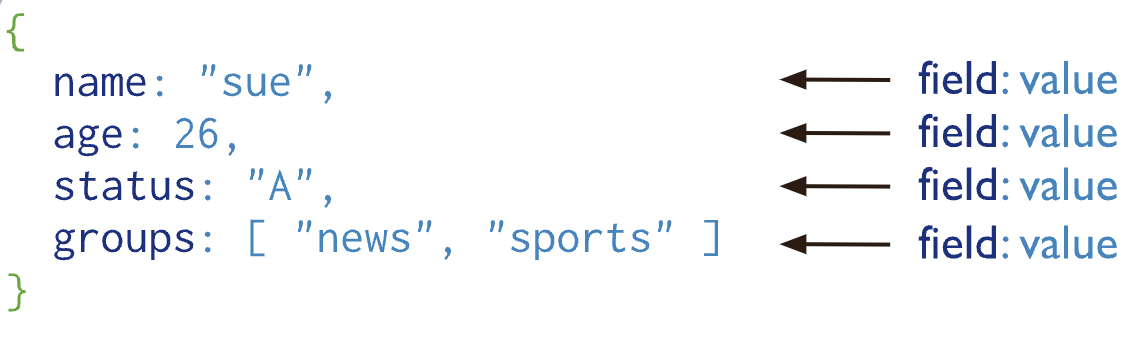
\includegraphics[width=0.8\textwidth]{pics/document.png}
    \caption{Document in MongoDB}
    \cite{mongodb_document}
    \label{fig:enter-label}
\end{figure}

Der Vorteil von Documents sind:
\begin{itemize}
    \item Dokumente entsprechen in einigen Programmiersprachen nativen Datentypen
    \item Die Einbindung von Arrays und Documents vermeidet aufwendige JOINS
    \item Durch das dynamische Schema kann man die Datenbankstruktur sehr vielseitig gestalten
\end{itemize}